\documentclass{article}
\usepackage[T1]{fontenc}
\usepackage{lmodern}
\usepackage{graphicx}
\usepackage{amsmath,amssymb}
\usepackage[a4paper,margin=2cm]{geometry}
\usepackage[absolute,overlay]{textpos}
\setlength{\TPHorizModule}{1mm}
\setlength{\TPVertModule}{1mm}
\usepackage[indonesian]{babel}
\usepackage{hyperref}
\setlength{\emergencystretch}{2em}
% unit: Halaman 39

\begin{document}

% === Halaman 39 (llm) ===

\begin{itemize}
  \item Jika $b = s$, maka mode $CFB$ $b$-bit adalah sbb:
\end{itemize}

\vspace{109.89mm}

\vspace{10mm}
(a) Enkripsi

\vspace{103.95mm}

\vspace{40mm}
(b) Dekripsi

% deskripsi: Diagram alur proses enkripsi menggunakan mode Cipher Feedback (CFB) dengan b = s, menunjukkan penggunaan IV, blok enkripsi Ek, plaintext P, dan ciphertext C.
% bbox normalisasi: [0.2600, 0.1300, 0.9400, 0.5000]
\begin{textblock*}{142.80mm}(54.60mm,38.61mm)
\noindent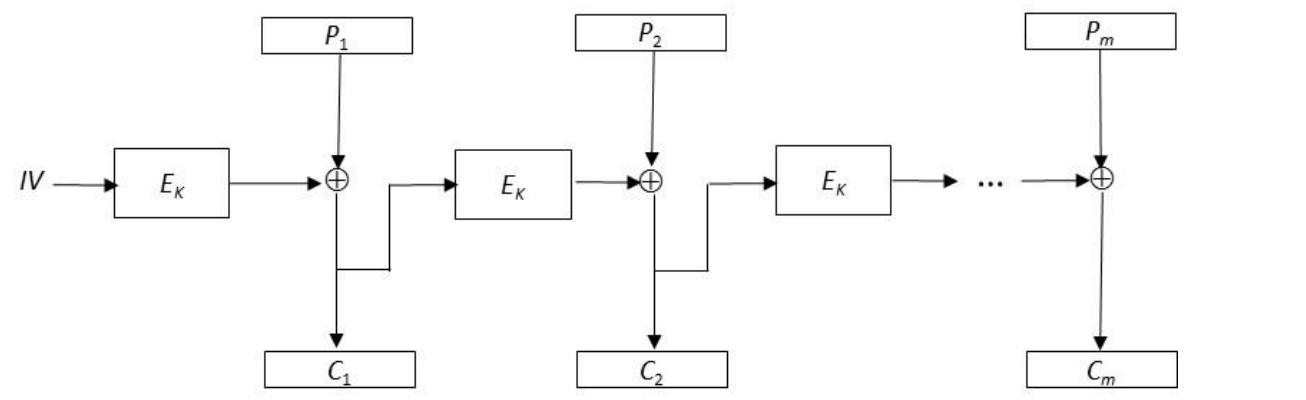
\includegraphics[width=142.80mm,height=109.89mm]{../../images/llm/page_039_img_01.png}%
\end{textblock*}

% deskripsi: Diagram alur proses dekripsi menggunakan mode Cipher Feedback (CFB) dengan b = s, menunjukkan bagaimana ciphertext C digunakan sebagai input untuk menghasilkan plaintext P.
% bbox normalisasi: [0.2600, 0.5800, 0.9400, 0.9300]
\begin{textblock*}{142.80mm}(54.60mm,172.26mm)
\noindent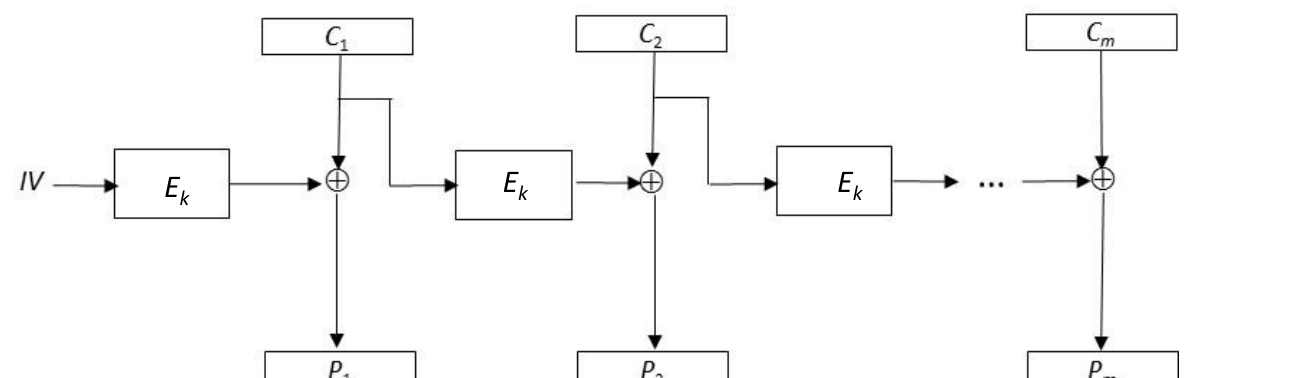
\includegraphics[width=142.80mm,height=103.95mm]{../../images/llm/page_039_img_02.png}%
\end{textblock*}

\end{document}
